\documentclass{article}
\usepackage{amsmath, amssymb, cite, algorithmic, url, braket}
\usepackage{graphicx}
\usepackage{pythonhighlight}
\usepackage[margin=1.5cm]{geometry}
\usepackage[title]{appendix}
\usepackage{listings}
\usepackage{booktabs}

\graphicspath{{../pic/}}
\lstset{
language=[ANSI]{C},
showtabs=true,
tab=,
tabsize=2,
basicstyle=\ttfamily\footnotesize,%\setstretch{.5},
stringstyle=\color{stringcolour},
showstringspaces=false,
alsoletter={1234567890},
otherkeywords={\%, \}, \{, \&, \|},
keywordstyle=\color{keywordcolour}\bfseries,
upquote=true,
morecomment=[s]{/*}{*/},
commentstyle=\color{commentcolour}\slshape,
literate=*%
{=}{{\literatecolour=}}{1}%
{-}{{\literatecolour-}}{1}%
{+}{{\literatecolour+}}{1}%
{*}{{\literatecolour*}}{1}%
{!}{{\literatecolour!}}{1}%
{[}{{\literatecolour[}}{1}%
{]}{{\literatecolour]}}{1}%
{<}{{\literatecolour<}}{1}%
{>}{{\literatecolour>}}{1}%
% {>>>}{\pythonprompt}{3}%
,%
frame=trbl,
rulecolor=\color{black!40},
backgroundcolor=\color{white},
breakindent=.5\textwidth,frame=single,breaklines=true
}

\begin{document}
\title{DSP Homework 04}
\author{Xu, Minhuan}
\maketitle
\tableofcontents
\begin{abstract}


\end{abstract}

\section{Problem 1}

\section{Problem 2}
\subsection{Problem Restatement}
When studying the sampling process, we use the function
\begin{equation}
    s(t) \quad = \quad \left\{ 
        \begin{array}{lr}
            1, & \mathrm{if}\; t = nT,\\
            0, & \mathrm{otherwise.}
        \end{array}
    \right.
\end{equation}
to express the sampling signal
\begin{align}
    x_s(t) \quad &= \quad x(t)s(t)\\
    &= \quad \left\{
        \begin{array}{lr}
            x(nT), & \mathrm{if}\; t = nT,\\
            0, & \mathrm{otherwise.}
        \end{array}
    \right.
\end{align}
It turns out that such approach is not useful when using the Fourier transform because
\begin{equation}
    \widetilde{s}(f) = \widetilde{x_s}(f) = 0 
    \label{ans}
\end{equation}
Prove (\ref{ans}).
\subsection{Prove}
According to the convolution theorem
\begin{equation*}
    \mathcal{F}\left[ x(t)*y(t) \right] = \widetilde{x}(f) \times \widetilde{y}(f)
\end{equation*}
if 
\begin{equation}
    \widetilde{s}(f) = 0
    \label{sub_ans}
\end{equation}
it's easy to prove Equation \ref{ans}.
I will prove Equation (\ref{sub_ans}) below. Easy to know that
\begin{align*}
    \widetilde{s}(t) &= \int_{-\infty}^{\infty} s(t) e^{-j2\pi ft} \mathrm{d}t\\
    &= \sum_{n = -\infty}^{\infty} e^{-j2\pi ft} \mathrm{d}t
\end{align*}
Because $n \in Z$, threfore
$$
\left\{
    \begin{array}{rl}
    e^{-j2\pi ft} &< \infty\\
    d(nT) &= 0
    \end{array}
\right.
$$
Therefore
\begin{equation*}
    \widetilde{s}(t) = \sum_{n = -\infty}^{\infty} 0 = 0
\end{equation*}
Therefore
\begin{equation*}
    \widetilde{x}_s(t) = \widetilde{s}(t) = 0
\end{equation*}
Equation (\ref{ans}) proved.
\section{Problem 3}
\subsection{Problem Restatement}
Design and carry out an experiment to find out the highest and lowest audio frequencies that your left and right ears can
hear.
\subsection{Preparation}
I followed the practice of Su Rundong to write a program to generate sound wave (sine wave) of specific frequency, and I think if I can use Qt Designer to generate a program with GUI.

Please look at Fig.\ref{UI}. If I want change the frequency of the sine wave, I can push the buttons or input the frequency I want into the lineEdit box. Push the start button to play the sound.

\begin{figure}[htbp]
    \centering
    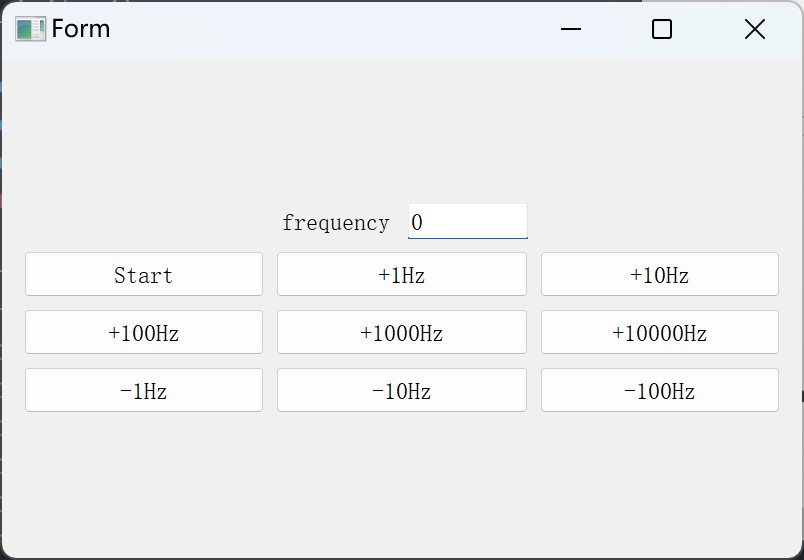
\includegraphics[keepaspectratio,width=250pt]{FreqWindow.jpg}
    \caption{UI of my program}\label{UI}
\end{figure}

\subsection{Interference Factors Elimination}
Earphone makers always tell us that human ears can hear $20-20\mathrm{k}~\mathrm{(Hz)}$. So, I must refer to the instructions of my earphones, and I find that they can only produce sound wave between $20-20\mathrm{k}~\mathrm{(Hz)}$, but actually I can hear some strange sounds if I turn the volumn to maximum. When I am testing my ears with 10$~\mathrm{Hz}$, what I hear cannot be the sound wave of 10$~\mathrm{Hz}$. 

I think it is from the mechanically collision, but I am not sure.To avoid this, I will first make the volumn of my earphones fixed.So I find a website\cite{HearingTest} to test my ears' frequency response, see Fig.\ref{FR}. The position of that black box is higher, I can hear that frequency harder. I don't want to hurt my ears, so I play a sound which is $1\mathrm{~kHz}$, then I will find out the exact range of the frequency my ears can hear in that volumn.

\begin{figure}[htbp]
    \centering
    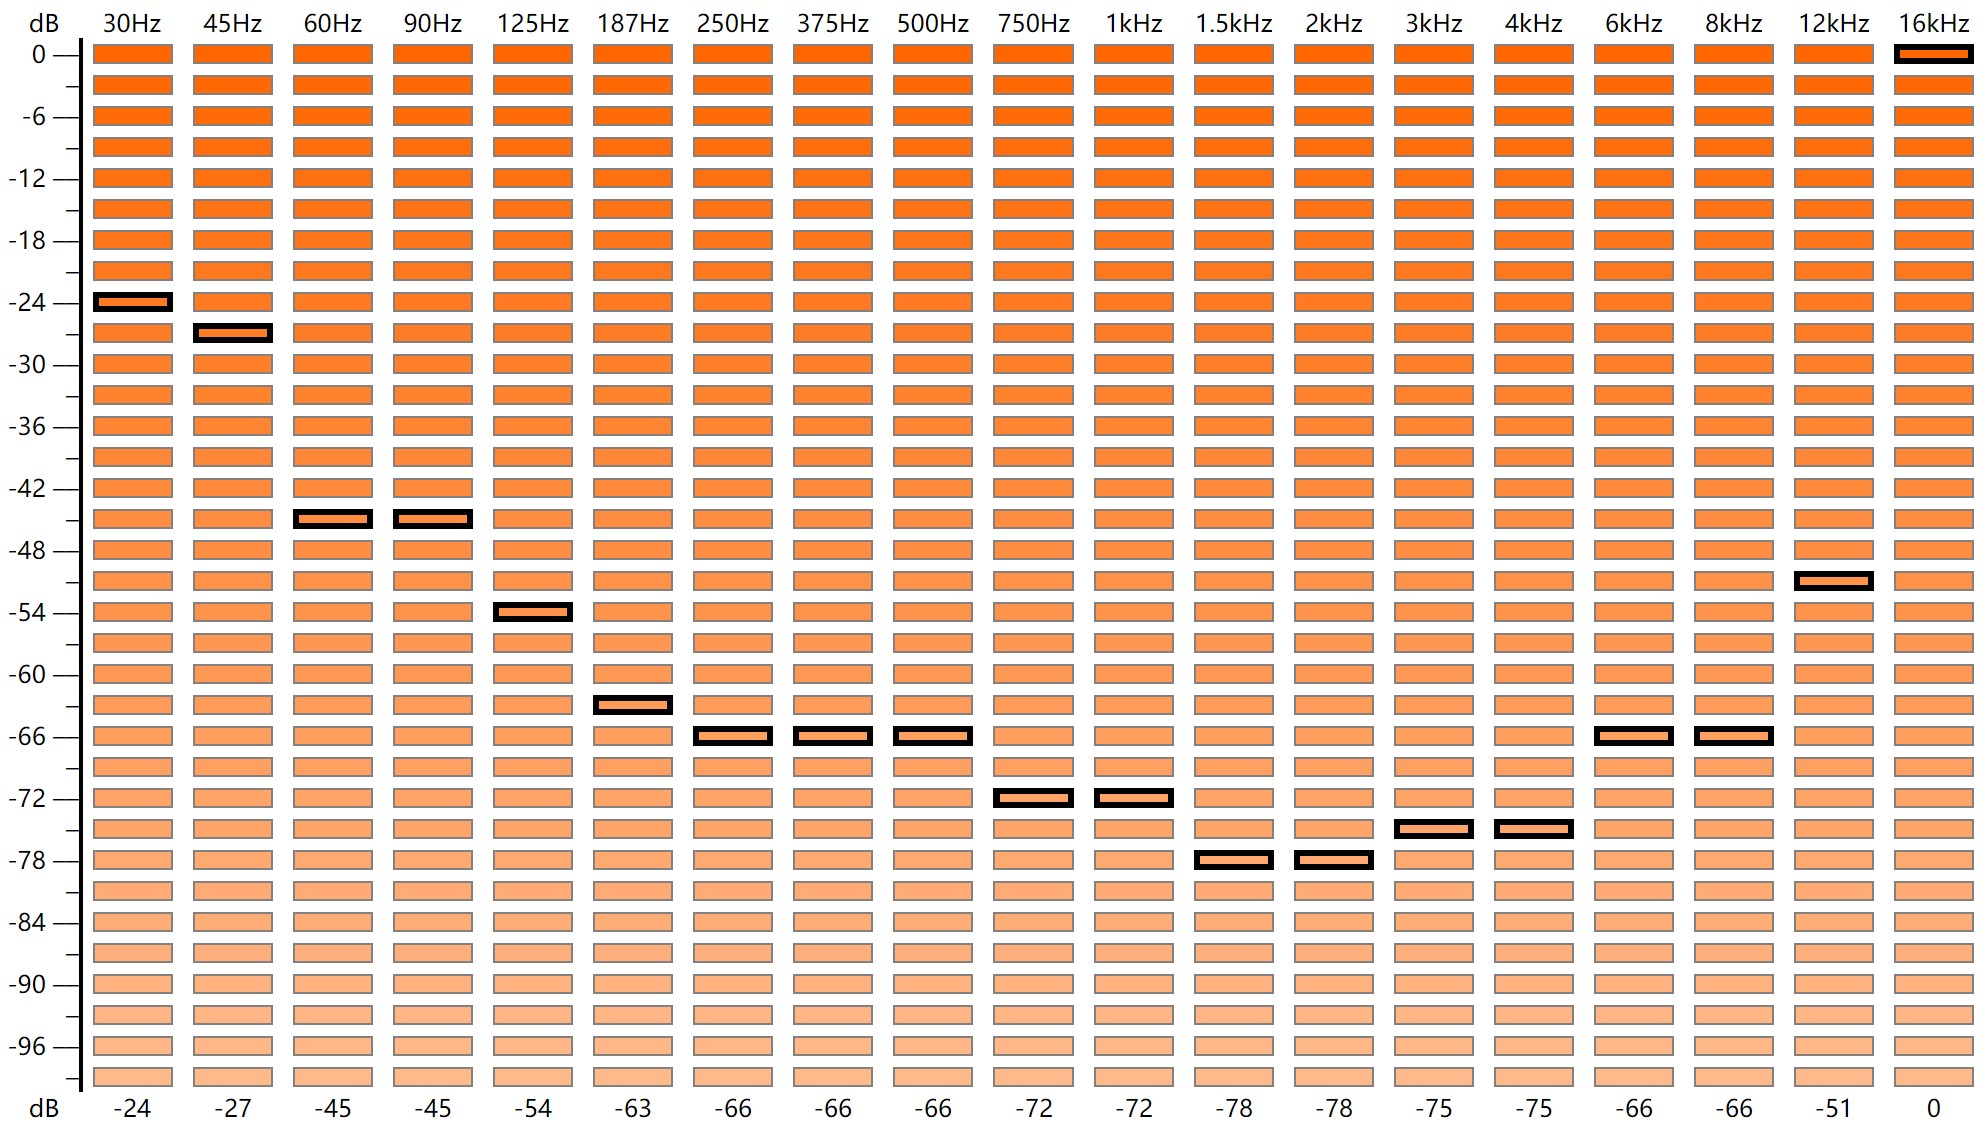
\includegraphics[keepaspectratio,width=400pt]{freqReaction.jpg}
    \caption{Frequency Response}
    \label{FR}
\end{figure}

\subsection{Implement}
From $1~\mathrm{kHz}$, I made the frequency higher and lower until I cannot hear the sound.
At last, in this way, the frequency response range of my ears is $xx \sim xx ~ \mathrm{kHz}$.


\bibliographystyle{ieeetr}
\bibliography{../bib/database}

\begin{appendices}
    \section{Code Listing}
    \begin{python}
    # main.py
    from PyQt5.QtWidgets import QApplication, QWidget
    import sys
    import sounddevice as sd
    import numpy as np
    from form import Ui_Form

    class FormWidget(QWidget):
        def __init__(self):
            super().__init__()
            self.ui = Ui_Form()
            self.ui.setupUi(self)
            self.ui.retranslateUi(self)
            self.Ui_connect()
            self.ui.freq_le.setText('0')
        
        def Ui_connect(self):
            self.ui.start.pressed.connect(self.toPlay)
            self.ui.m1.pressed.connect(self.addFreq)
            self.ui.m10.pressed.connect(self.addFreq)
            self.ui.m100.pressed.connect(self.addFreq)
            self.ui.p1.pressed.connect(self.addFreq)
            self.ui.p10.pressed.connect(self.addFreq)
            self.ui.p100.pressed.connect(self.addFreq)
            self.ui.p1000.pressed.connect(self.addFreq)
            self.ui.p10000.pressed.connect(self.addFreq)

        def toPlay(self):
            f = int(self.ui.freq_le.text()) #Hz
            fs = 96000 #Hz
            length = 10 #s
            x = np.arange(fs*length)
            y0 = np.zeros(fs*length)
            y = np.sin(2 * np.pi * f / fs * x)
            sd.play(y,fs,blocking=False)
            
        def addFreq(self):
            sender = self.sender()
            sender_name = sender.objectName()
            try:
                f = int(self.ui.freq_le.text())
            except:
                self.ui.freq_le.setText('0')
                f = 1
            if sender_name == 'm1':
                f = f - 1
            elif sender_name == 'm10':
                f = f - 10
            elif sender_name == 'm100':
                f = f - 100
            elif sender_name == 'p1':
                f = f + 1
            elif sender_name == 'p10':
                f = f + 10
            elif sender_name == 'p100':
                f = f + 100
            elif sender_name == 'p1000':
                f = f + 1000
            else:
                f = f + 10000
            self.ui.freq_le.setText(str(f))
            

    if __name__ == '__main__':
        app = QApplication(sys.argv)
        main = FormWidget()
        main.show()
        sys.exit(app.exec_())
    \end{python}
    \begin{python}
    #form.py

    
    # -*- coding: utf-8 -*-

    # Form implementation generated from reading ui file 'form.ui'
    #
    # Created by: PyQt5 UI code generator 5.15.7
    #
    # WARNING: Any manual changes made to this file will be lost when pyuic5 is
    # run again.  Do not edit this file unless you know what you are doing.


    from PyQt5 import QtCore, QtGui, QtWidgets


    class Ui_Form(object):
        def setupUi(self, Form):
            Form.setObjectName("Form")
            Form.resize(800, 500)
            self.verticalLayout = QtWidgets.QVBoxLayout(Form)
            self.verticalLayout.setObjectName("verticalLayout")
            self.gridLayout = QtWidgets.QGridLayout()
            self.gridLayout.setObjectName("gridLayout")
            self.freq_lb = QtWidgets.QLabel(Form)
            self.freq_lb.setAlignment(QtCore.Qt.AlignCenter)
            self.freq_lb.setObjectName("freq_lb")
            self.gridLayout.addWidget(self.freq_lb, 0, 1, 1, 1)
            self.freq_le = QtWidgets.QLineEdit(Form)
            self.freq_le.setObjectName("freq_le")
            self.gridLayout.addWidget(self.freq_le, 0, 2, 1, 1)
            self.start = QtWidgets.QPushButton(Form)
            self.start.setObjectName("start")
            self.gridLayout.addWidget(self.start, 1, 0, 1, 1)
            self.p1 = QtWidgets.QPushButton(Form)
            self.p1.setObjectName("p1")
            self.gridLayout.addWidget(self.p1, 1, 1, 1, 2)
            self.p10 = QtWidgets.QPushButton(Form)
            self.p10.setObjectName("p10")
            self.gridLayout.addWidget(self.p10, 1, 3, 1, 1)
            self.m1 = QtWidgets.QPushButton(Form)
            self.m1.setObjectName("m1")
            self.gridLayout.addWidget(self.m1, 3, 0, 1, 1)
            self.p100 = QtWidgets.QPushButton(Form)
            self.p100.setObjectName("p100")
            self.gridLayout.addWidget(self.p100, 2, 0, 1, 1)
            self.p1000 = QtWidgets.QPushButton(Form)
            self.p1000.setObjectName("p1000")
            self.gridLayout.addWidget(self.p1000, 2, 1, 1, 2)
            self.p10000 = QtWidgets.QPushButton(Form)
            self.p10000.setObjectName("p10000")
            self.gridLayout.addWidget(self.p10000, 2, 3, 1, 1)
            self.m10 = QtWidgets.QPushButton(Form)
            self.m10.setObjectName("m10")
            self.gridLayout.addWidget(self.m10, 3, 1, 1, 2)
            self.m100 = QtWidgets.QPushButton(Form)
            self.m100.setObjectName("m100")
            self.gridLayout.addWidget(self.m100, 3, 3, 1, 1)
            self.gridLayout.setColumnStretch(0, 2)
            self.gridLayout.setColumnStretch(1, 1)
            self.gridLayout.setColumnStretch(2, 1)
            self.gridLayout.setColumnStretch(3, 2)
            self.verticalLayout.addLayout(self.gridLayout)

            self.retranslateUi(Form)
            QtCore.QMetaObject.connectSlotsByName(Form)

        def retranslateUi(self, Form):
            _translate = QtCore.QCoreApplication.translate
            Form.setWindowTitle(_translate("Form", "Form"))
            self.freq_lb.setText(_translate("Form", "frequency"))
            self.start.setText(_translate("Form", "Start"))
            self.p1.setText(_translate("Form", "+1Hz"))
            self.p10.setText(_translate("Form", "+10Hz"))
            self.m1.setText(_translate("Form", "-1Hz"))
            self.p100.setText(_translate("Form", "+100Hz"))
            self.p1000.setText(_translate("Form", "+1000Hz"))
            self.p10000.setText(_translate("Form", "+10000Hz"))
            self.m10.setText(_translate("Form", "-10Hz"))
            self.m100.setText(_translate("Form", "-100Hz"))
    \end{python}
\end{appendices}



\end{document}

